\subsection*{PGL: Prior-Guided Local Self-supervised Learning
for 3D Medical Image Segmentation}

% \subsubsection*{Ссылка} \url{https://arxiv.org/abs/2011.12640}
\subsubsection*{Введение}
В данной работе \cite{ann15} предланается self-supervised модель Prior-Guided Local (PGL) 
для сегментации трехмерных медицинских изображений, которая использует изначально
известное расположение между парой позитивных изображений, чтобы выявить местную 
зависимость признаков в одном и том же регионе.
\subsubsection*{Основная идея}
Предложенная модель состоит из модуля аугментации данных для генерации 
представлений изображения и модуля известного двойного пути (prior dual-path module)
для извлечения признаков. Далее конструируется функция потерь местных зависимостей, 
для минимизации различий между каждой парой выявленных признаков. Таким образом, модель
учится захватывать больше структурной информации и больше подходит для решения задачи сегментации, 
чем методы, основанные на выявлении глобальных зависимостей. 
\par 
\textbf{Отличие метода PGL от BYOL} \par
\textit{Bootstrap Your Own Latent (BYOL)} - метод, в котором сеть 
обучается онлайн на представлениях изображений для того, чтобы предсказать вид
следующего представления. BYOL фокусируется на изучении глобальных зависимостей между 
парой представлений, в то время как PGL использует априорную информацию о
взаимном расположении двух представлений, чтобы извлечь локальные зависимости в одинаковых регионах.


\begin{minipage}{1.0\linewidth}
    \begin{center}
        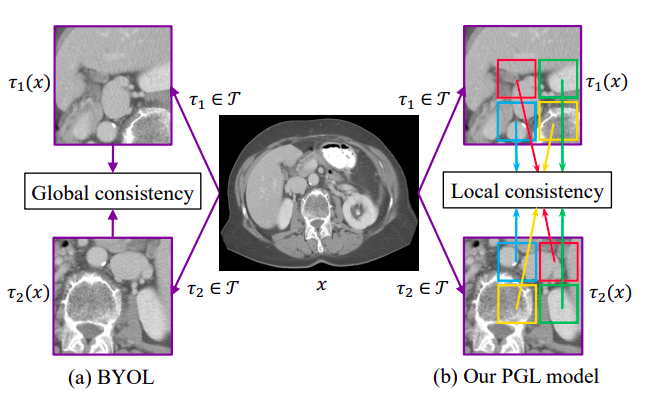
\includegraphics[scale=0.5]{ann15_byol.png} \\
        % \caption{\scriptsize{BYOL и PGL}}
    \end{center}
\end{minipage}
\\
\begin{minipage}{1.0\linewidth}
    \begin{center}
        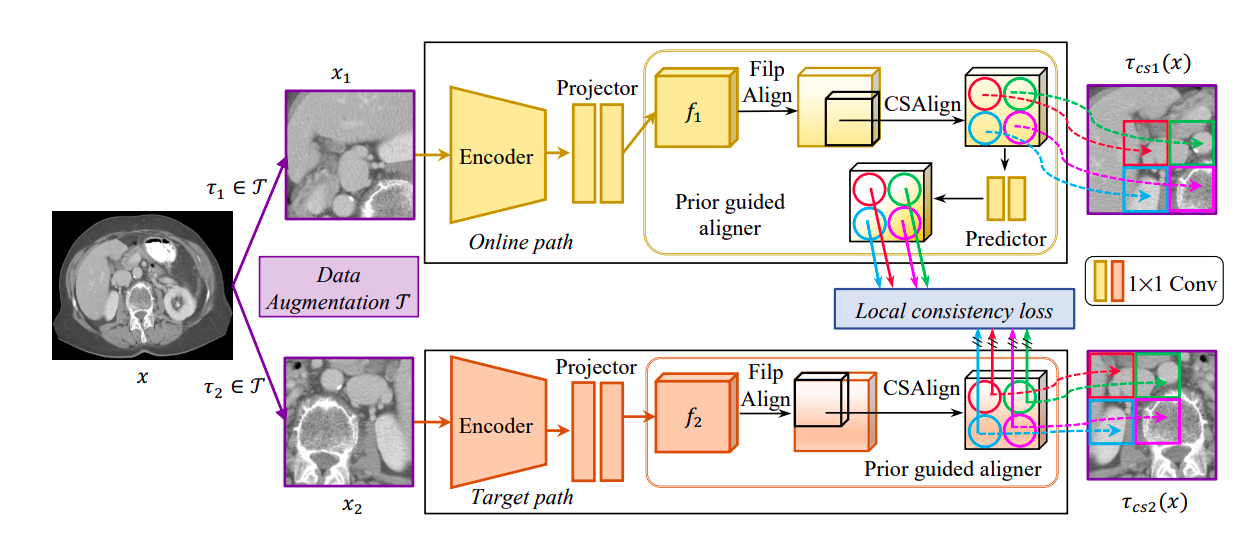
\includegraphics[scale=0.35]{ann15_arch.png} \\
        % \caption{\scriptsize{Архитектура PGL}}
    \end{center}
\end{minipage}
\subsubsection*{Данные}
Liver,Spleen,KiTS, BCV из Medical Segmentation
Decathlon (MSD) соревнования, RibFac датасет.
\subsubsection*{Результаты}
Производительность baseline сети с использованием случайной инициализации или одной из трех 
стратегий предобучения: Models Genesis (MG), BYOL и  PGL на датасете BCV:

\begin{minipage}{1.0\linewidth}
    \begin{center}
        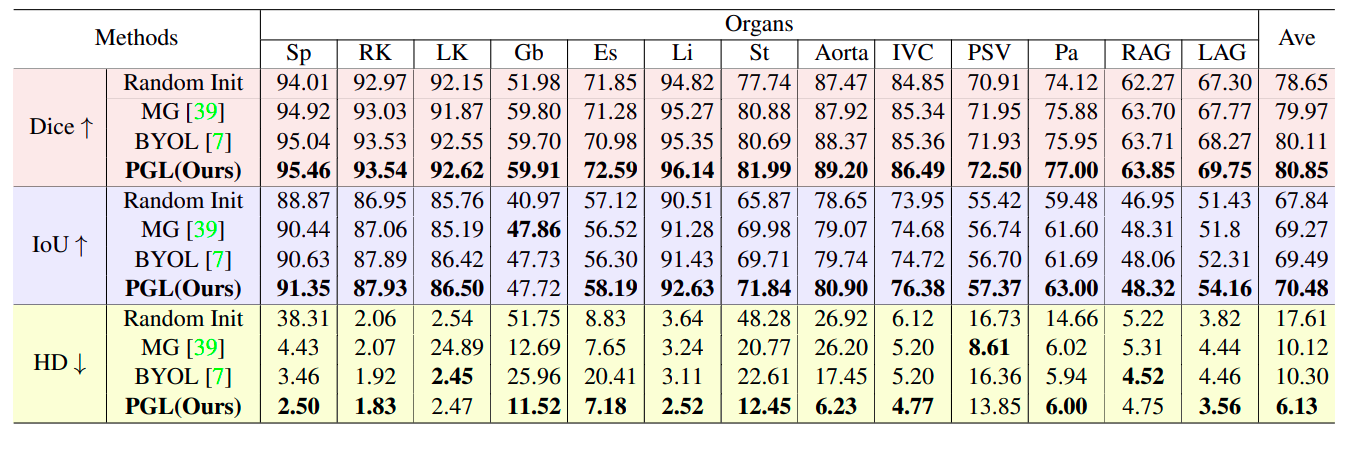
\includegraphics[scale=0.35]{ann15_res.png} \\
        % \caption{\scriptsize{Результаты предсказания моделей на датасете BCV. Ave - 
        % средний результат сегментации 13 органов.}}
    \end{center}
\end{minipage}


\begin{minipage}{0.49\linewidth}
    \begin{center}
        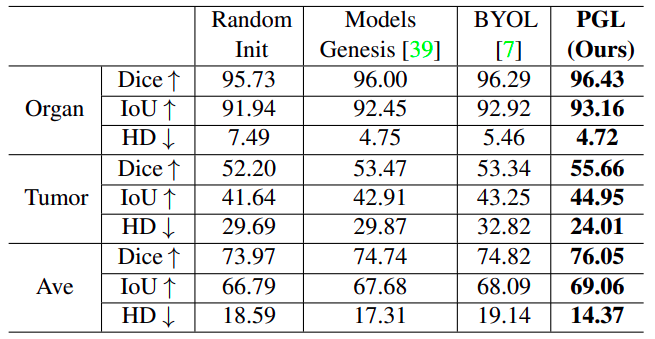
\includegraphics[scale=0.35]{ann15_res2.png} \\
        % \caption{\scriptsize{
        %     Производительность PGL модели с различными пространственными 
        %     трансформациями на датасете Liver. Ave - 
        %     средний результат сегментации печени и опухоли печени.
        % }}
    \end{center}
    
\end{minipage}
\begin{minipage}{0.49\linewidth}
    \begin{center}
        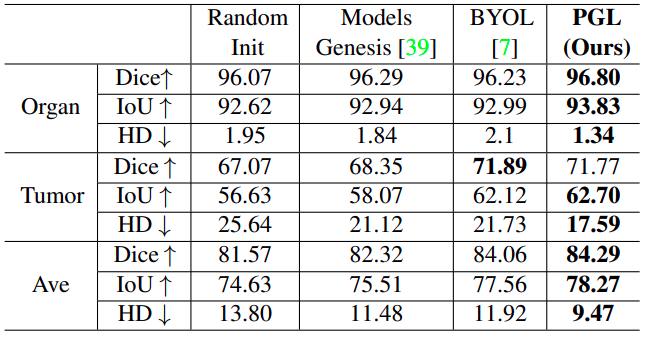
\includegraphics[scale=0.35]{ann15_res3.png} \\
        % \caption{\scriptsize{Производительность PGL модели с 
        % различными пространственными 
        % трансформациями на датасете KiTS. Ave - 
        % средний результат сегментации почек и опухолей почек.}}
    \end{center}
    
\end{minipage} 


\subsubsection*{Заключение}
Были проведены масшатбные эксперименты на четырех КТ датасетах, которые включали в себя 
11 органов и два вида опухолей. Результаты показали, что использование PGL для инифиализации 
сети для сегментации позволяет сильно улучшить производительность сети, также показано 
превосходство предложенной модели PGL над моделью BYOL.